%================ch3======================================
\chapter{Analysing the data}\label{ch:ch3}

\section{Radial Distribution of Stars}
The radial distributions were calculated for each cluster individually for each track. The mean shift algorithm was used to find the center of the clusters. The celestial coordinates of the center of the cluster allows us to calculate the radial distance of every star in the cluster from its center. The \lstinline{astropy.coordinates} {}submodule has some useful classes in this regard. We can get the radial separation of these stars from the cluster center in arcminutes.

\subsection{Mean Shift Algorithm}
The mean shift algorithm is an unsupervised, non-parametric, clustering algorithm. It iteratively shifts points towards the highest density of data points - cluster centers - and classifies them accordingly. It doesn't make any assumption about the model like K-means or Gaussian mixture models. The \lstinline{scikit-learn}\citep{scikit-learn} implementation was used. The model takes in a parameter - bandwidth. This bandwidth is used in the RBF kernel for the algorithm. This parameter defines how many clusters will be there in the data. Setting a relatively high value for this makes sure there is only one cluster in the data. 

\subsection{Plotting the Distributions}
The calculated radial distance was plotted against the number of stars under that distance for a single track and a binary track. 

\begin{figure}[H]
\centering
\begin{subfigure}[b]{0.4\textwidth}
  \centering
  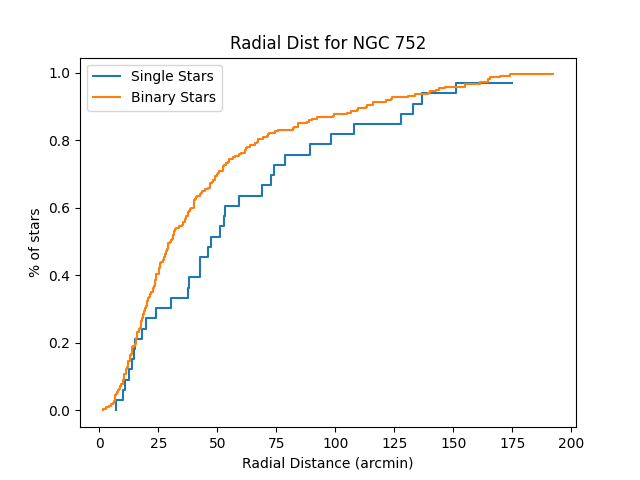
\includegraphics[width=\textwidth]{NGC 752_rad.png}
  \caption{NGC 752}
  \label{fig:im4}
 \end{subfigure}
~
\begin{subfigure}[b]{0.4\textwidth}
  \centering
  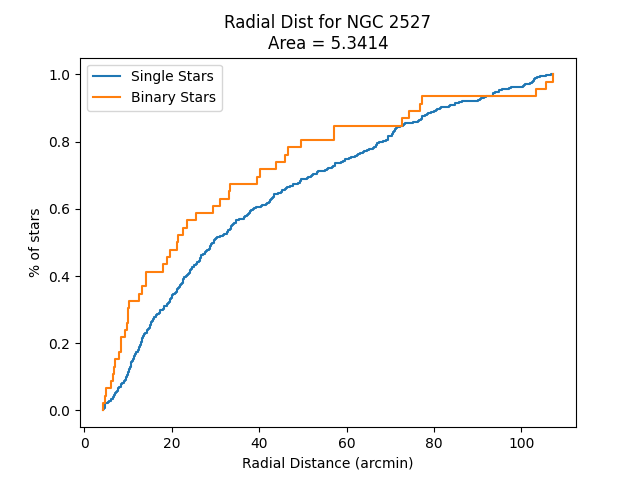
\includegraphics[width=\textwidth]{NGC 2527_rad.png}
  \caption{NGC 2527}
  \label{fig:im5}
\end{subfigure}
\caption{Radial Distribution for Star Clusters}
\label{fig:sim1}
\end{figure}

\section{King's Profile}
The King's profile\citep{kingprofile} is fitted for all the clusters in the study. The stars are divided into bins based on the radial distance from the cluster center. These bins are all annular rings of equal areas. This would mean the $n^{th}$ bin would be sandwiched between rings of radius $\sqrt{n-1}R$ and $\sqrt{n}R$ where $R$ is the radius of the cluster. After finding the number of stars in one bin, dividing that number by the area of the ring gives the surface density. When plotted against the radius on a log-log plot, we get a distribution of stars based on their proximities to the cluster center. Now we fit the curve given by the following equation to the data.
$$f = k \left( \frac{r_c}{\sqrt{r^2+r_c^2}} - \frac{r_t}{\sqrt{r_c^2+r_t^2}} \right) ^2$$
$k$ is an amplitude or a scaling factor, $r_c$ is the core radius and $r_t$ is the tidal radius. $k$ is simply the surface density of the innermost bin. $r_c$ and $r_t$ are the variable parameters which can be modified to get the best fit to the data. From the fitting procedure we can determine the core radius and tidal radius of the star cluster. The profile can be plotted easily with the \lstinline{astropy}\citep{astropy} module.

\section{Determining Mass Function}
The mass of stars in the main sequence is strongly correlated with the magnitude of the stars. This relation can be found by fitting a polynomial to our data. \lstinline{numpy} {}has a submodule for dealing with polynomials and the \lstinline{polyfit} {}will fit a polynomial to the given data. In this study, we attempted to fit a cubic polynomial to approximate the relationship between magnitude and mass. 

\begin{figure}[h]
	\centering
	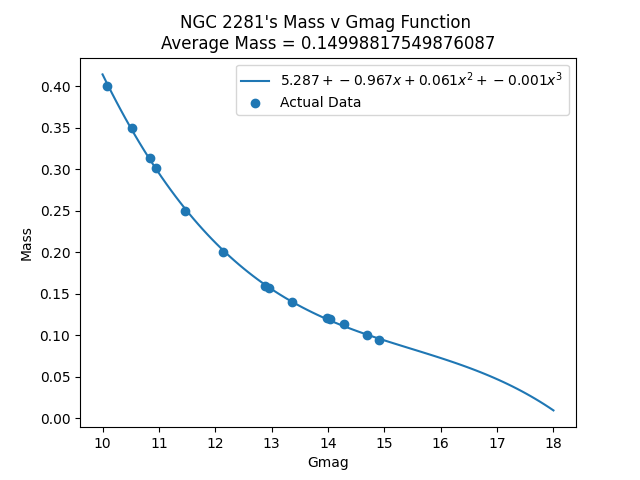
\includegraphics[width=0.6\linewidth]{NGC 2281_mass_dist.png}
	\caption{Fitting the polynomial for the isochrone of NGC 2281}
	\label{fig:im6}
\end{figure}

\subsection{Central Density}
To determine the central density, we will consider the stars in a small radius around the center of the cluster. We will first convert the radius of this region into parsecs to calculate the volume using the standard formula for the volume of a sphere. Next, we will sum up the estimated masses of all the stars in this region. This can be done by finding the mass by substituting the known magnitude values into the mass function estimated by the isochrone. Now that we have evaluated both the mass of the center and its volume, we can find the central density.

\section{Determing the Relaxation Time for the Clusters}
With the average mass, number of stars in the cluster, central density and cluster radius, we have found out all the parameters we need to find the relaxation time. We can use this equation to evalute the same.
$$t_{rc} = 1.491 \times 10^7 \text{yr} \times \frac{k}{\ln(0.4 N_*)} <m_*>^{-1} \rho_{M, 0}^{1/2} r_c^3$$

Finally, since all the stars along the isochrone are of similar age, we can use the isochrone age as an approximation for the age of the entire cluster. In combination with the calculated time, this allows us to identify the relaxations the cluster has undergone.

$$N_{relax} = C_{Age}/t_{rc}$$
